% !TEX program = pdflatex
% ============================================================================
% Problem Set 1 - Section 1: Age-Labor Income Profile
% Slide deck. Every number and figure is pulled from output/ so the deck stays
% in sync with script/04_age_labor_income.r: re-run that script, recompile this
% file, done. Nothing is hard-coded here.
%
%   - \input ../../output/tables/age_income_stats.tex        (numbers as macros)
%   - \input ../../output/tables/age_income_slide_table.tex  (regression table)
%   - ../../output/figures/age_income_profile.png            (fitted profiles)
%   - ../../output/figures/income_dist_age.png               (descriptive motivation)
%
% Compile from inside presentation/:  pdflatex age_income_slides.tex
% Export/submit as age_equipo_XX.pdf (XX = team number; see \teamnumber below).
% ============================================================================
\documentclass[aspectratio=169]{beamer}

\usepackage[utf8]{inputenc}
\usepackage[T1]{fontenc}
\usepackage[spanish,es-noshorthands]{babel}
\usepackage{booktabs}
\usepackage{graphicx}
\usepackage{amsmath}
\usepackage{xcolor}

% uandespurple: deck accent (frame titles, structure). specuncond/speccond
% match the two curves in the age-income profile figure (04_age_labor_income.r)
% so the spec labels below carry the same colour as the plot.
\definecolor{uandespurple}{HTML}{6C0A8A}
\definecolor{specuncond}{HTML}{235DA3}
\definecolor{speccond}{HTML}{AD0D5D}

\usetheme{Boadilla}
\setbeamercolor{structure}{fg=uandespurple}
\setbeamercolor{frametitle}{fg=uandespurple}
\setbeamercolor{title}{fg=uandespurple}
\setbeamertemplate{navigation symbols}{}
\setbeamertemplate{caption}[numbered]
\setbeamerfont{frametitle}{size=\large}

% Key numbers (peak ages, bootstrap CIs, R^2, N, ...) as LaTeX macros.
\newcommand{\AgePeakUncond}{40.7}
\newcommand{\AgePeakUncondLo}{40.2}
\newcommand{\AgePeakUncondHi}{41.3}
\newcommand{\AgePeakCond}{43.6}
\newcommand{\AgePeakCondLo}{42.9}
\newcommand{\AgePeakCondHi}{44.4}
\newcommand{\AgeRsqUncond}{0.052}
\newcommand{\AgeRsqCond}{0.227}
\newcommand{\AgeNobs}{14,763}
\newcommand{\AgeBootReps}{5,000}
\newcommand{\AgeBetaAge}{0.087}
\newcommand{\AgeBetaAgeSq}{-0.00107}


\newcommand{\teamnumber}{XX}

\title[Perfil edad--ingreso]{Perfil edad--ingreso laboral en Bogotá}
\subtitle{Problem Set 1 \textbullet\ Sección 1 }
\author[Perez, Lozano, Suarez]{María José Pérez \and Juan Manuel Lozano \and Samuel Suárez Valle}
\institute[Uniandes]{MECA 4107 --- Big Data y Machine Learning para Economía Aplicada}
\date{Septiembre 2026}

\begin{document}

\begin{frame}[plain]
  \titlepage
\end{frame}

% ---------------------------------------------------------------------------
% Slide 1 (mandatory): Result Overview
% ---------------------------------------------------------------------------
\begin{frame}{Resultado principal}
  \begin{block}{El ingreso laboral crece con la edad, alcanza un máximo y luego decae}
    \begin{itemize}
      \item \textbf{Perfil incondicional}
        $\bigl(\log w = \beta_1 + \beta_2\,\text{edad} + \beta_3\,\text{edad}^2 + u\bigr)$:
        edad pico \textbf{\AgePeakUncond\ años},
        IC bootstrap 95\% $[\AgePeakUncondLo,\ \AgePeakUncondHi]$,
        \ $R^2 = \AgeRsqUncond$.
      \item \textbf{Perfil condicional} (añade horas trabajadas y tipo de empleo):
        edad pico \textbf{\AgePeakCond\ años},
        IC 95\% $[\AgePeakCondLo,\ \AgePeakCondHi]$,
        \ $R^2 = \AgeRsqCond$.
      \item El máximo cae \emph{dentro} del rango de edad observado (Q3) y demuestra que la edad nos permite aproximar una apreciación y posterior depreciación del ingreso laboral en la vida adulta.
    \end{itemize}
  \end{block}
  \vfill
  {\footnotesize IC estimado por bootstrap con \AgeBootReps\ repeticiones (remuestreo de
  individuos). Muestra: \AgeNobs\ ocupados de 18 años o más con ingreso laboral positivo,
  ponderada por \texttt{fex\_c}.}
\end{frame}

% ---------------------------------------------------------------------------
\begin{frame}{Pregunta y marco teórico}
  \textbf{¿Cómo varía el ingreso laboral a lo largo del ciclo de vida en Bogotá,
  y qué le dice ese perfil a la autoridad tributaria?}
  \vspace{0.6em}
  \begin{itemize}
    \item Teoría del capital humano (Mincer, 1974): los retornos a la experiencia son
      decrecientes $\Rightarrow$ el perfil edad--ingreso es cóncavo.
      \begin{itemize}
      \item La inversión en capacitación disminuye mientras disminuye el tiempo para recuperar los costos.
      \item El deterioro cognitivo causa mayores depreciaciones de las habilidades con la edad.
      \item El conocimiento técnico adquirido en primeros años se hace obsoleto.
      \end{itemize}
    \item Especificación cuadrática en la edad captura esa concavidad y nos da edad pico: $\text{edad}^\ast = -\beta_2 / (2\beta_3)$.
    \item En tributación: el perfil fija un ingreso esperado por edad; desviaciones
      sistemáticas por debajo de ese perfil son una señal (más no evidencia contundente) de posible sub-reporte.
  \end{itemize}
\end{frame}

% ---------------------------------------------------------------------------
\begin{frame}{Datos y decisiones empíricas}
  \begin{itemize}
    \item \textbf{Fuente:} GEIH 2018 (Bogotá), 10 \emph{chunks} scrapeados y combinados.
    \item \textbf{Muestra:} ocupados de 18 años o más (\texttt{age >= 18 \& ocu == 1}).
    \item \textbf{Variable dependiente:} $\log$ del ingreso laboral mensual total
      (\texttt{y\_total\_m} $=$ asalariado $+$ independiente).
    \item \textbf{Ponderación:} todas las regresiones usan \texttt{fex\_c}
      (factor de expansión).
  \end{itemize}
\end{frame}

% ---------------------------------------------------------------------------
\begin{frame}{Evidencia descriptiva: Ingresos medios y pico}
  \centering
  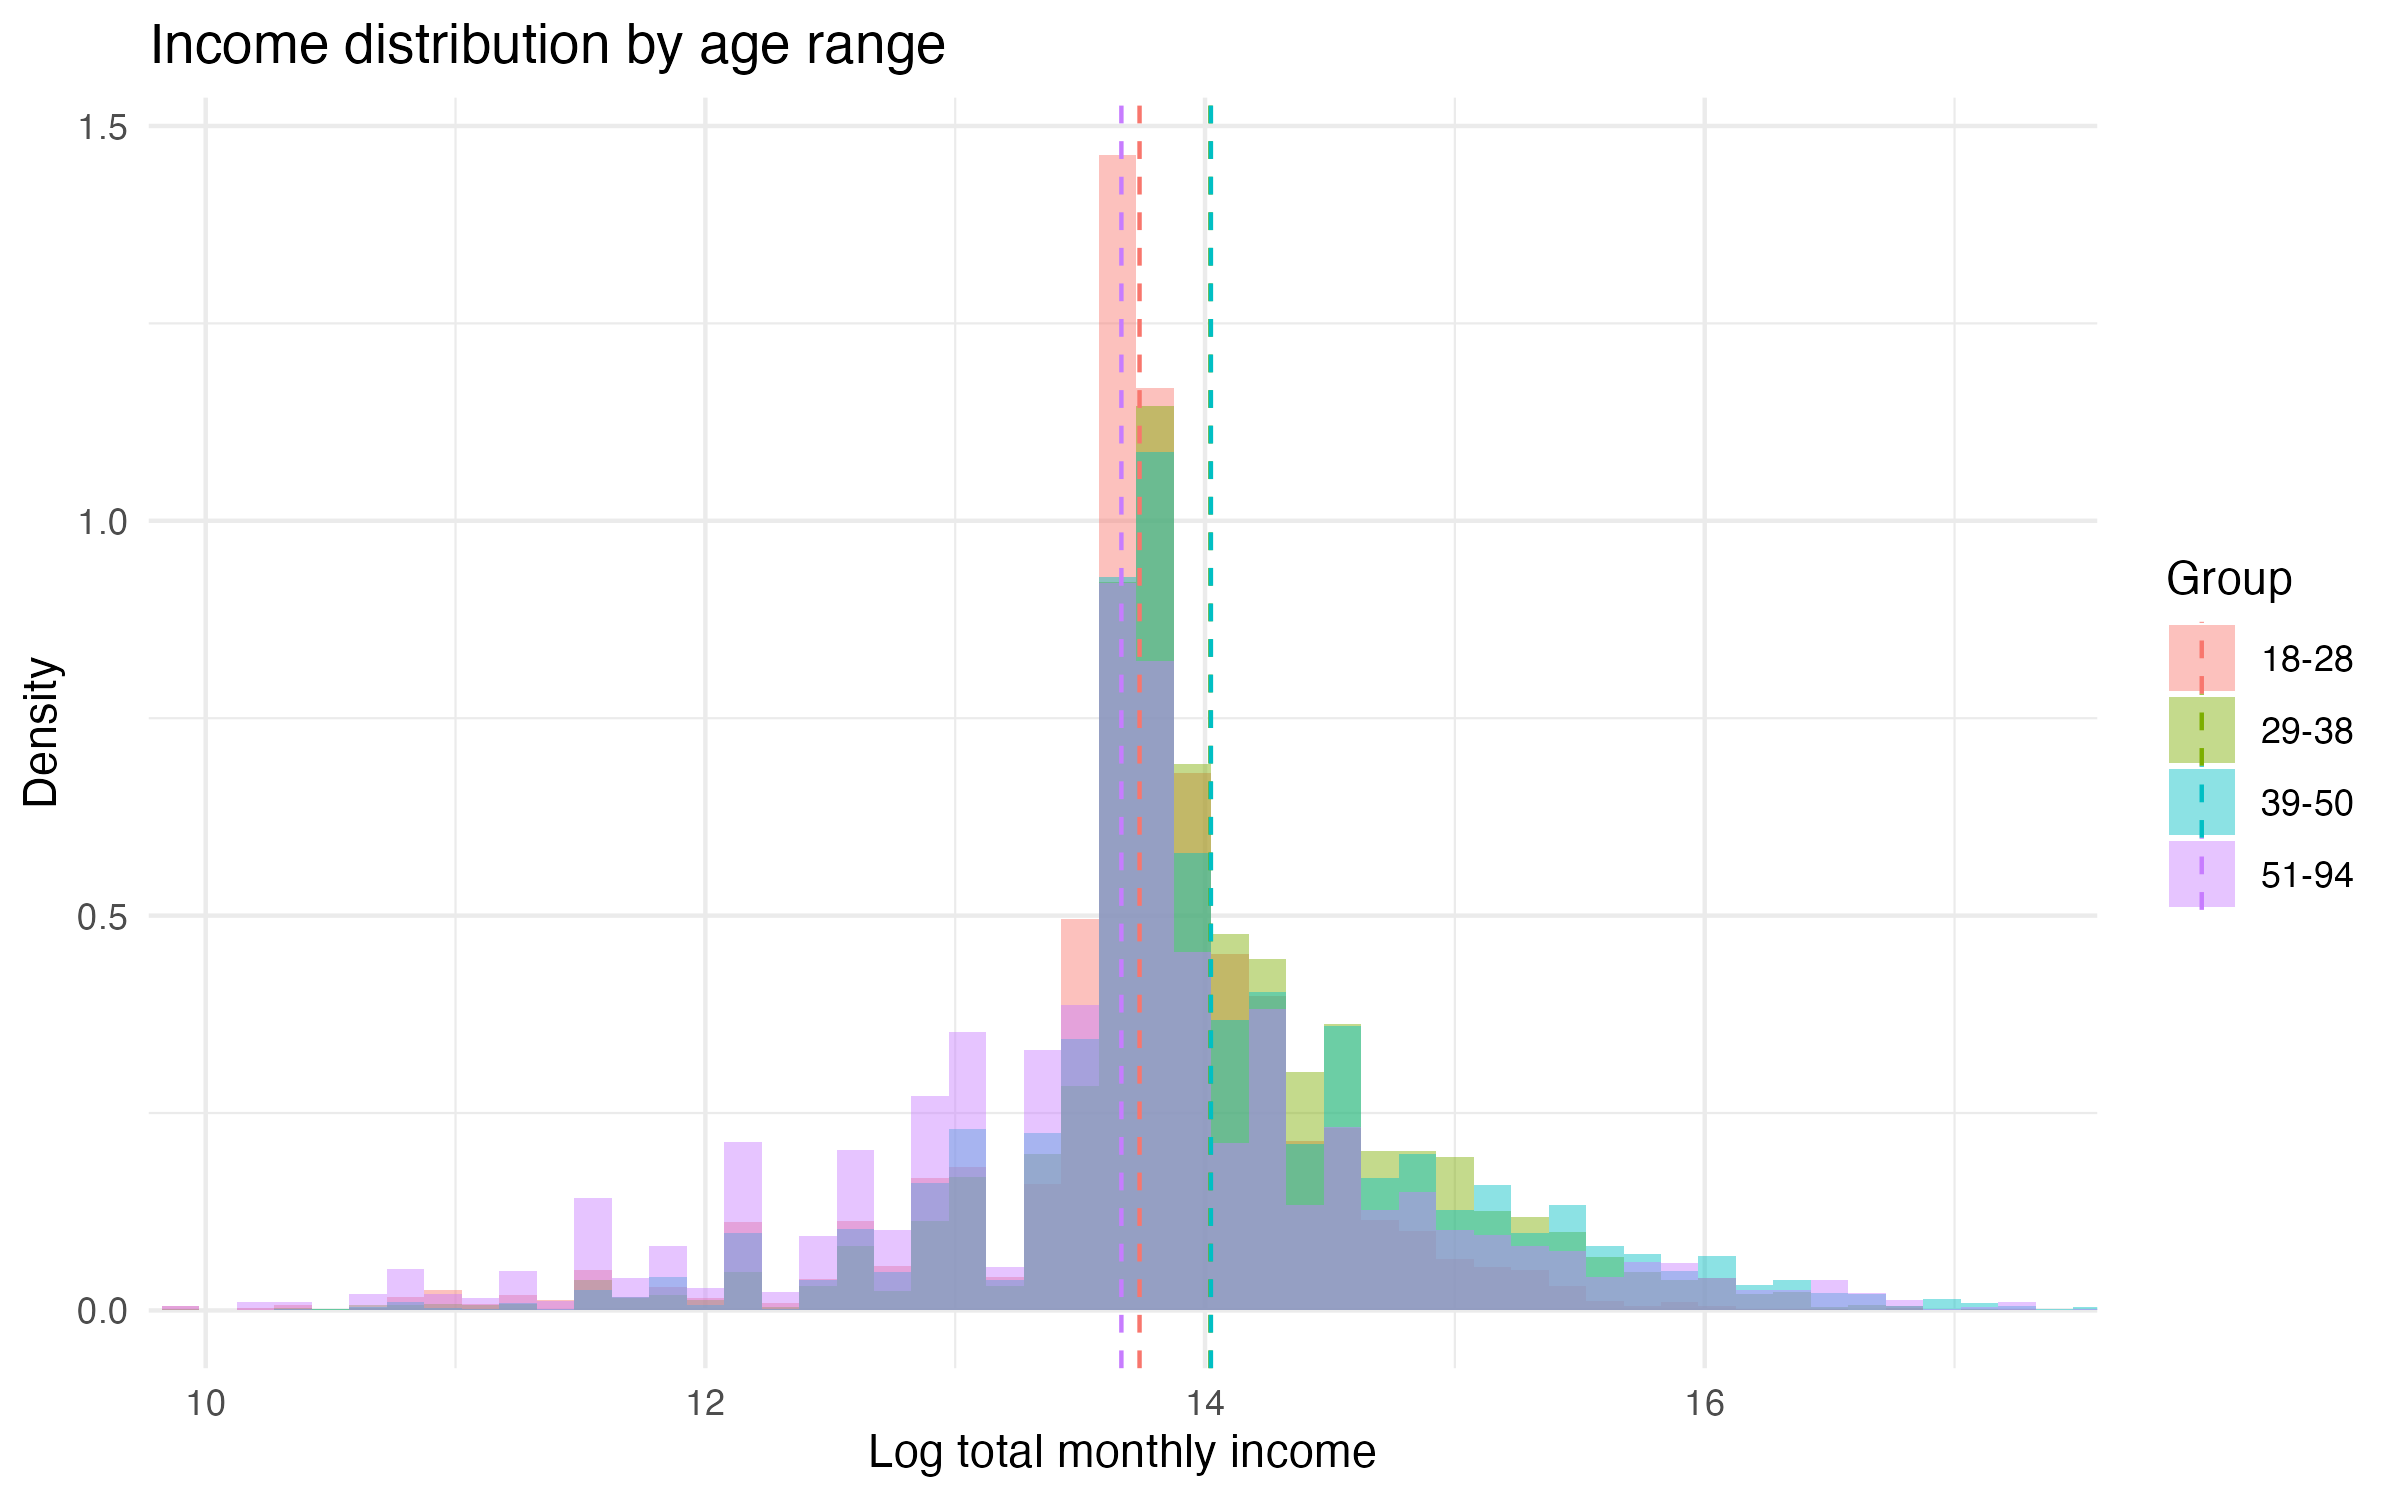
\includegraphics[height=0.80\textheight]{../../output/figures/income_dist_age.png}

  {\footnotesize Líneas punteadas: media ponderada de $\log$ ingreso por rango de
  edad. La media sube de 18--28 a 29--38, se estanca en 39--50 (prácticamente
  empatada con 29--38) y retrocede en 51--94: igual que el perfil.}
\end{frame}

% ---------------------------------------------------------------------------
\begin{frame}{Especificaciones}
  \textbf{Incondicional}
  \[
    \log(w_i) = \beta_1 + \beta_2\,\text{edad}_i + \beta_3\,\text{edad}_i^2 + u_i
  \]

  \textbf{Condicional}
  \[
    \log(w_i) = \beta_1 + \beta_2\,\text{edad}_i + \beta_3\,\text{edad}_i^2
      + \gamma\,\text{horas}_i + \sum_{k}\delta_k\,\text{relab}_{k,i} + u_i
  \]

  \vspace{0.4em}
  \begin{itemize}
    \item Edad pico implícita: $\text{edad}^\ast = -\beta_2 / (2\beta_3)$
      (cóncava, dado $\beta_3 < 0$).
    \item IC del pico por \textbf{bootstrap}: \AgeBootReps\ remuestreos de individuos,
      reestimando en cada uno la misma especificación ponderada; percentiles 2.5 y 97.5
      de la distribución de $\text{edad}^\ast$.
  \end{itemize}
\end{frame}

% ---------------------------------------------------------------------------
\begin{frame}{Comparación de especificaciones}
  \centering
  {\small 
\begin{tabular}[t]{lcc}
\toprule
 & Unconditional & Conditional\\
\midrule
Age & 0.087 (0.003) & 0.073 (0.003)\\
Age$^2$ & -0.001066 (0.000038) & -0.000841 (0.000035)\\
Total hours worked (per month) &  & 0.0127 (0.0004)\\
Employment type (relab) fixed effects & No & Yes\\
\midrule
Implied peak age & 40.7 & 43.6\\
\addlinespace
95\% bootstrap CI for peak age & {}[40.2, 41.3] & {}[42.9, 44.4]\\
$R^2$ & 0.052 & 0.227\\
N & 14,764 & 14,764\\
\bottomrule
\end{tabular}
}

  \vspace{0.6em}
  {\footnotesize Errores estándar entre paréntesis. Regresiones ponderadas por
  \texttt{fex\_c}. Los efectos fijos de tipo de empleo (\texttt{relab}) se incluyen
  pero no se reportan individualmente. IC del pico: percentil bootstrap 95\%.}
\end{frame}

% ---------------------------------------------------------------------------
\begin{frame}{Perfiles edad--ingreso estimados}
  \centering
  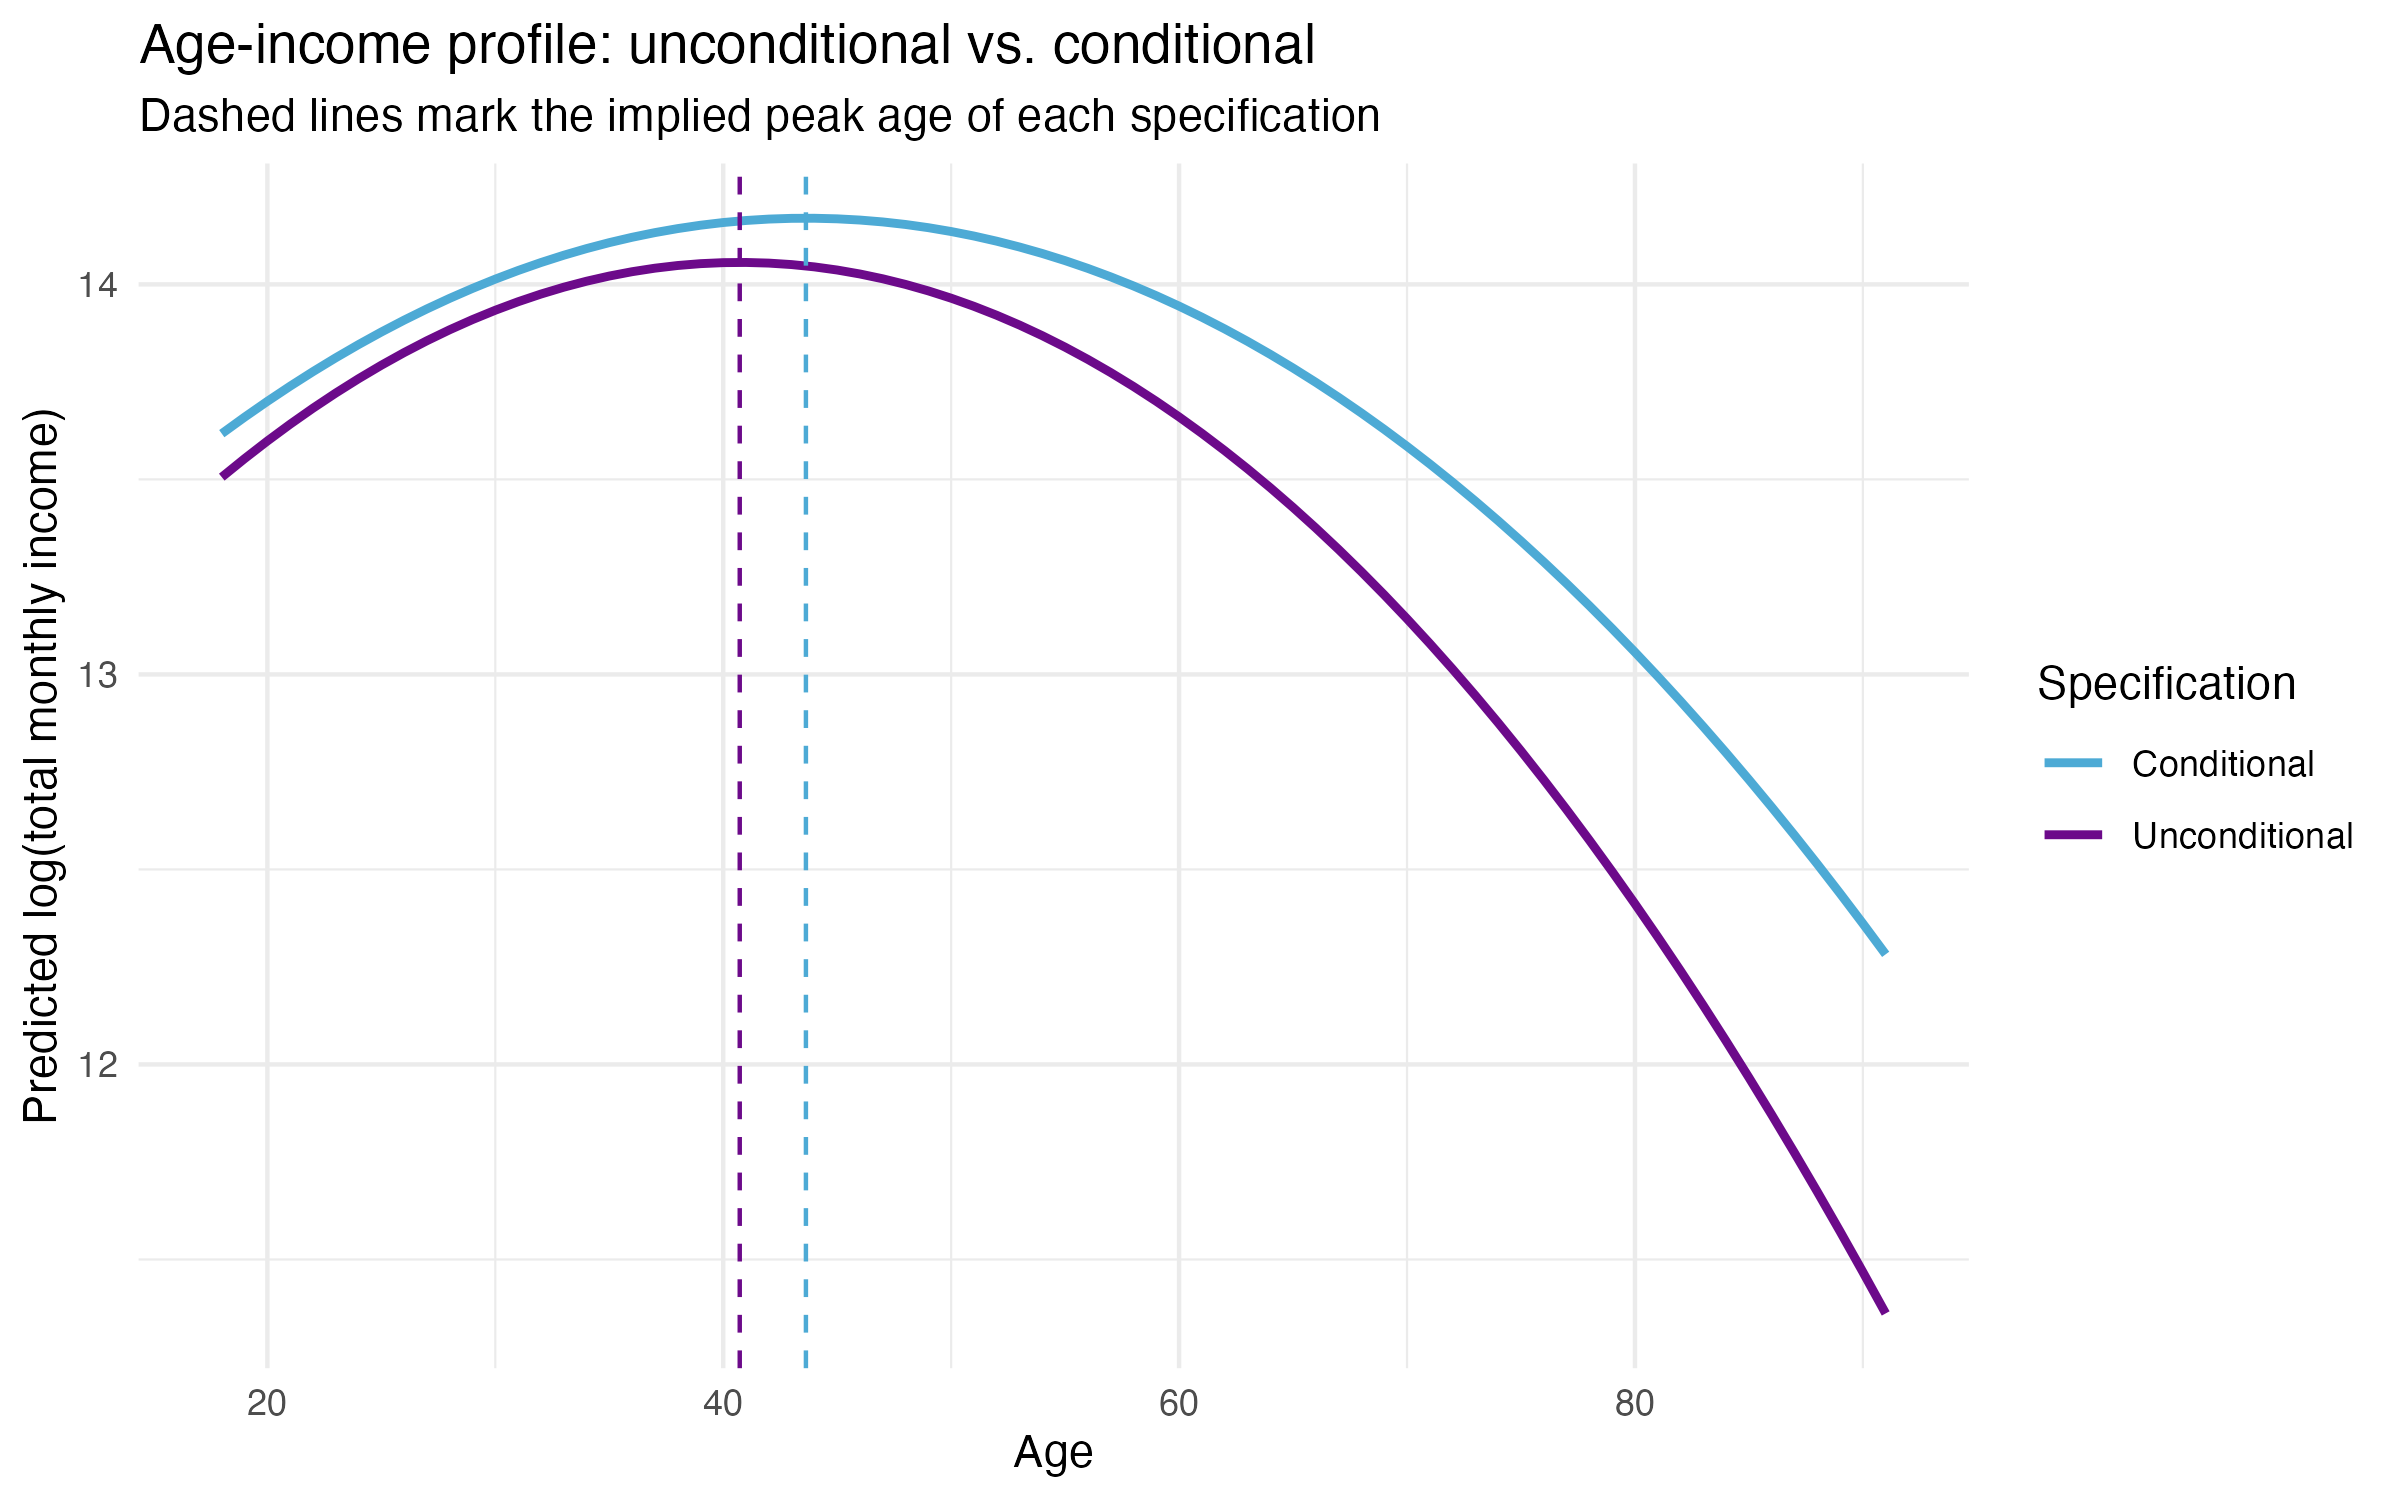
\includegraphics[height=0.78\textheight]{../../output/figures/age_income_profile.png}

  {\footnotesize Líneas punteadas: edad pico implícita de cada especificación;
  bandas sombreadas: su IC bootstrap 95\%. Eje vertical en escala logarítmica,
  etiquetado en pesos. Del perfil condicional no interpretamos su \emph{altura}
  (nivel de ingreso, que depende de las categorías base de horas y tipo de
  empleo): solo su \emph{ancho} (concavidad) y la \emph{edad pico}.}
\end{frame}

% ---------------------------------------------------------------------------
\begin{frame}{Edad pico e intervalo de confianza}
  \begin{columns}[T]
    \begin{column}{0.42\textwidth}
      \textcolor{specuncond}{\textbf{Incondicional}}
      \begin{itemize}
        \item Edad pico: \textbf{\AgePeakUncond\ años}
        \item IC 95\%: $[\AgePeakUncondLo,\ \AgePeakUncondHi]$
        \item $R^2 = \AgeRsqUncond$
      \end{itemize}
      \vspace{0.6em}
      \textcolor{speccond}{\textbf{Condicional}}
      \begin{itemize}
        \item Edad pico: \textbf{\AgePeakCond\ años}
        \item IC 95\%: $[\AgePeakCondLo,\ \AgePeakCondHi]$
        \item $R^2 = \AgeRsqCond$
      \end{itemize}
    \end{column}
    \begin{column}{0.56\textwidth}
      \begin{itemize}
        \item Intervalos estrechos ($\approx 1$ año de ancho) y dentro del rango de edad observado.
        \item Al condicionar por horas y tipo de empleo, la edad pico se
          \textbf{desplaza hacia edades mayores} ($\approx +3$ años) y el perfil
          se aplana.
        \item Al controlar, la edad pierde sus efectos indirectos $\Rightarrow$ la curva se ensancha:
          \begin{itemize}
            \item \textbf{Horas de trabajo:} a edades extremas se trabaja menos tiempo.
            \item \textbf{Tipo de empleo:} a edades extremas se trabaja en modalidades de menor ingreso.
          \end{itemize}
      \end{itemize}
    \end{column}
  \end{columns}
\end{frame}

% ---------------------------------------------------------------------------
\begin{frame}{Conclusiones}
  \begin{itemize}
    \item El perfil edad--ingreso en Bogotá es cóncavo, con un pico entre los
      \textbf{\AgePeakUncond\ y \AgePeakCond\ años}, consistente con la teoría del
      capital humano.
    \item El pico se estima con \textbf{precisión} (IC bootstrap estrecho), pero el
      $R^2$ es \textbf{bajo} ($\AgeRsqUncond$ / $\AgeRsqCond$): la edad explica poco
      de la varianza individual del ingreso.
    \item En contexto de tributación: la edad da una referencia de ingreso esperado
      por ciclo de vida, pero es un predictor débil. Es útil combinarla con
      horas, tipo de empleo y otras características (Secciones 2 y 3).
  \end{itemize}
\end{frame}

\end{document}
